\documentclass{beamer}
\usepackage{ctex, hyperref}
\usepackage[T1]{fontenc}

% other packages
\usepackage{latexsym,amsmath,xcolor,multicol,booktabs,calligra}
\usepackage{graphicx,pstricks,listings,stackengine}

\author{郑晖}
\title{基于 GRN 的垂体基因表达差异分析}
\subtitle{2021武汉大学本科毕业答辩}
\institute{武汉大学弘毅学堂}
\date{2021年5月13日}
\usepackage{WHU}

% defs
\def\cmd#1{\texttt{\color{red}\footnotesize $\backslash$#1}}
\def\env#1{\texttt{\color{blue}\footnotesize #1}}
\definecolor{deepblue}{rgb}{0,0,0.5}
\definecolor{deepred}{rgb}{0.6,0,0}
\definecolor{deepgreen}{rgb}{0,0.5,0}
\definecolor{halfgray}{gray}{0.55}

\lstset{
  basicstyle=\ttfamily\small,
  keywordstyle=\bfseries\color{deepblue},
  emphstyle=\ttfamily\color{deepred},    % Custom highlighting style
  stringstyle=\color{deepgreen},
  numbers=left,
  numberstyle=\small\color{halfgray},
  rulesepcolor=\color{red!20!green!20!blue!20},
  frame=shadowbox,
}


\begin{document}

\kaishu
\begin{frame}
  \titlepage
  \begin{figure}[htpb]
    \begin{center}
      
\includegraphics[width=0.2\linewidth]{logo/whu.eps}
    \end{center}
  \end{figure}
\end{frame}

\begin{frame}
  \tableofcontents[sectionstyle=show,subsectionstyle=show/shaded/hide,subsubsectionstyle=show/shaded/hide]
\end{frame}


\section{研究背景与内容}

\begin{frame}{研究背景}
  \begin{columns}
    \begin{column}{.5\linewidth}
      \begin{itemize}
        \item HPA 轴是体内的压力反应中心,连接中枢神经系统(CNS)和内分泌系统。
        \item 作为 HPA 轴组成部分的垂体,在炎症事件调节过程中起到重要的作用。
        \item 以往探究垂体在中枢神经内分泌炎症调节过程中作用的研究都没有涉及到单细胞转录层级。
      \end{itemize}
    \end{column}
 
    \begin{column}{.5\linewidth}
      \includegraphics<1>[width=\linewidth]{figs/HPA.png}
    \end{column}
  \end{columns}
\end{frame}

\begin{frame}{研究内容}
  \begin{itemize}
    \item 我们主要关注不同的垂体细胞如何响应炎症刺激,动态炎症研究将成为我们实验中最重要的部分。
    \item 我们将基于病毒或细菌感染建立炎症小鼠模型,并主要使用单细胞转录组测序以及数据分析和数据挖掘来找出炎症、垂体和激素之间的关系。
  \end{itemize}
\end{frame}

\section{相关工作}

\subsection{单细胞 RNA 测序}

\begin{frame}{单细胞 RNA 测序}
  \begin{columns}
    \begin{column}{.5\linewidth}
    单细胞 RNA 测序(scRNA­seq)技术提供了在单细胞水平观测基因表达的方法,可以更好地研究以下问题:
      \begin{itemize}
        \item 探究异质性
        \item 谱系路径分析
        \item 随机基因表达研究
      \end{itemize}
    \end{column}
 
    \begin{column}{.5\linewidth}
      \includegraphics<1>[width=\linewidth]{figs/scseq-purpose.png}
    \end{column}
  \end{columns}
\end{frame}

\begin{frame}{单细胞 RNA 测序数据处理流程}
  \begin{columns}
    \begin{column}{.5\linewidth}
      \setbeamercolor{alerted text}{fg=red}
      \begin{itemize}
        \item<1-|alert@1> 将原始测序数据转化为基因表达矩阵。
        \item<2-|alert@2> 对基因表达矩阵进行质量控制。
        \item<3-|alert@3> 依据基因表达矩阵进行聚类。
      \end{itemize}
    \end{column}

    \begin{column}{.5\linewidth}
      \includegraphics<1>[width=\linewidth]{figs/cellranger-workflow.png}
      \includegraphics<2>[width=\linewidth]{figs/qc-workflow.png}
      \includegraphics<3>[width=\linewidth]{figs/cluster-workflow.png}
    \end{column}
  \end{columns}
\end{frame}

\subsection{基因调控网络}

\begin{frame}{基因调控网络}
  \begin{itemize}
    \item 基因调控网络(GRN)定义并维持特定于细胞类型的转录状态,这反过来又是细胞形态和功能的基础。
    \item 基于大规模转录组和表观基因组数据来计算预测 GRN 是一个广泛研究的领域。相关算法包括GENIE3、GRNBoost2和BEELINE等,在这项研究中我们主要使用基于GRNBoost2的SCENIC,进行基因调控网络推断。
  \end{itemize}
  \center
  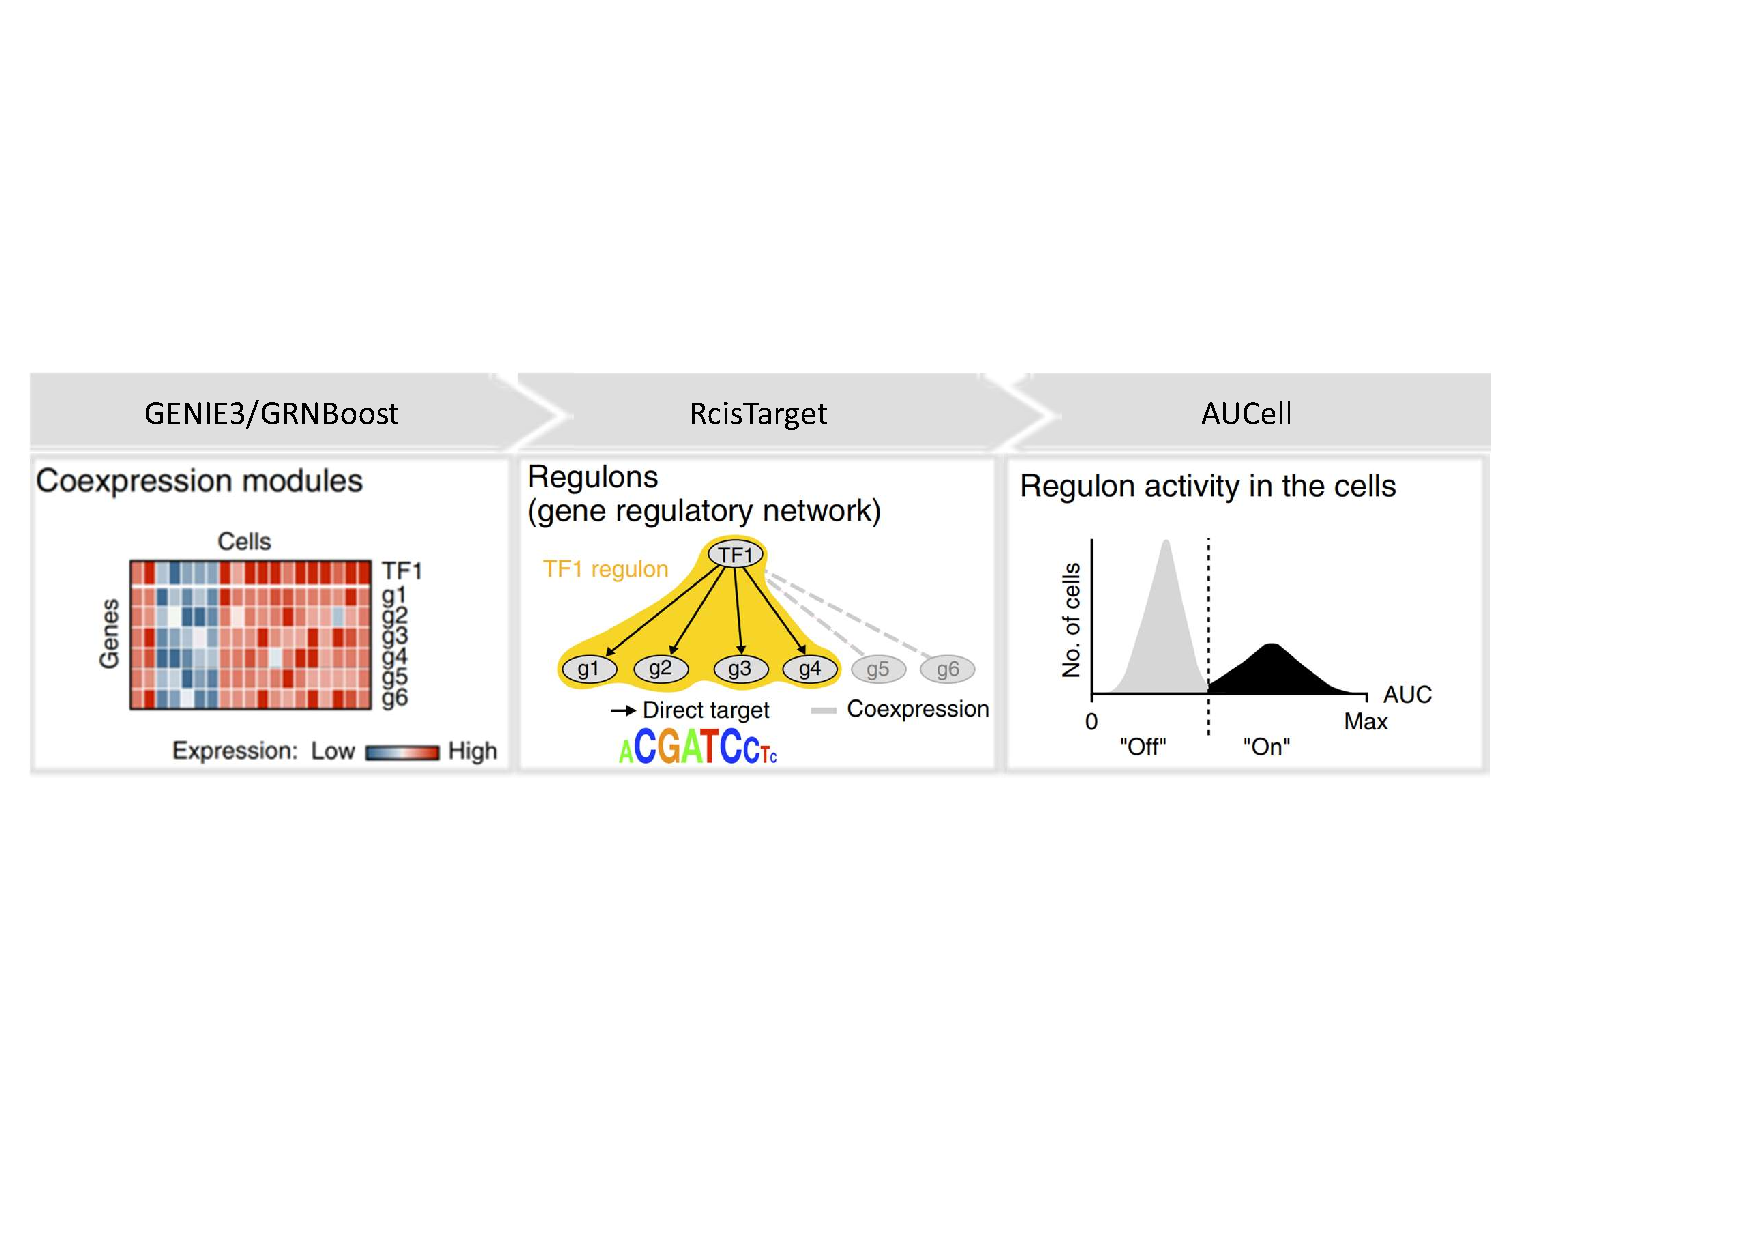
\includegraphics[width=0.8\linewidth]{figs/scenic-workflow.pdf}
\end{frame}

\section{实验设计流程}

\begin{frame}{实验设计流程}
  \begin{columns}
    \begin{column}{.5\linewidth}
      \setbeamercolor{alerted text}{fg=red}
      \begin{itemize}
        \item 建立一个涉及多种免疫刺激剂、多尺度给药剂量与恢复时程的小鼠炎症模型。
        \item 组织解离、梯度离心分离。
        \item 使用改进的Smart-seq2方法获得垂体单细胞转录组。
      \end{itemize}
    \end{column}

    \begin{column}{.5\linewidth}
      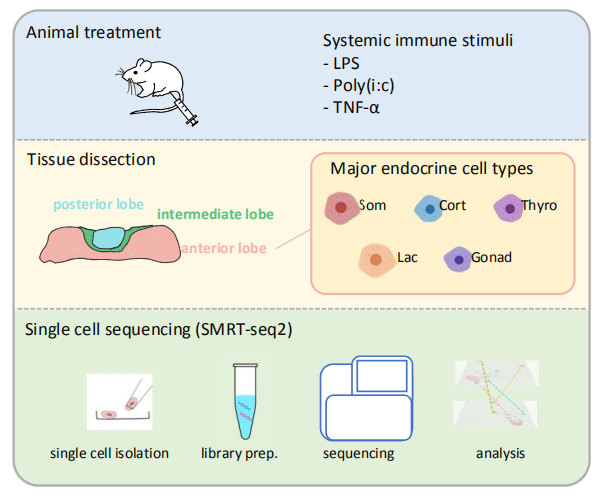
\includegraphics[width=\linewidth]{figs/expr-design.png}
    \end{column}
  \end{columns}
\end{frame}

\section{实验数据分析}

\subsection{测序数据预处理}

\begin{frame}{测序数据预处理}
  \begin{columns}
    \begin{column}{.5\linewidth}
      \setbeamercolor{alerted text}{fg=red}
      \begin{itemize}
        \item 对基因-细胞矩阵进行质量控制、降维可视化。
        \item 依据各细胞类型已知的基因marker对数据进行标注。
        \item 留下Som、Cort、Lac、Thyro以及Gonad五类细胞,进行进一步分析。
      \end{itemize}
    \end{column}

    \begin{column}{.5\linewidth}
      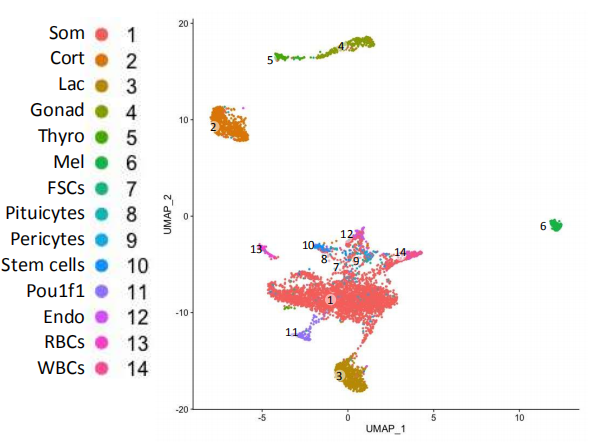
\includegraphics[width=\linewidth]{figs/expr-res1.png}
    \end{column}
  \end{columns}
\end{frame}

\subsection{测序数据SCENIC分析}

\begin{frame}{测序数据SCENIC分析}
  我们对筛选出来的测序数据进行 SCENIC 分析,以推断其潜在转录因子及对应目的基因。对输出的AUC-score矩阵进行降维聚类,并用其聚类结果作为细胞是否处于炎症状态的判别标准。
  \center
  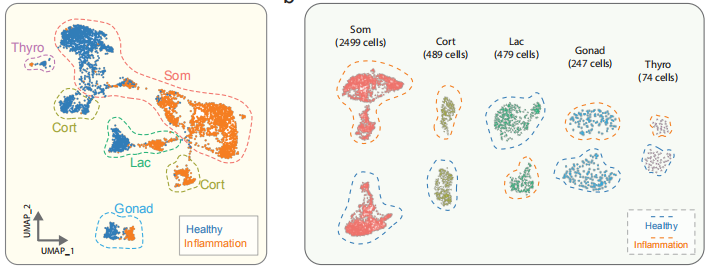
\includegraphics[width=0.8\linewidth]{figs/expr-res2.png}
\end{frame}

\begin{frame}{分析处理条件与垂体细胞状态之间的关系}
  \begin{columns}
    \begin{column}{.5\linewidth}
      \begin{itemize}
        \item 所有注射saline的处理组,基本都处于健康状态。
        \item 注射低剂量LPS或者经历了长时程的恢复的处理组,仅有少部分处于炎症状态。
        \item 注射高剂量LPS且仅经历短时程恢复的处理组则大多处于炎症状态。
      \end{itemize}
    \end{column}

    \begin{column}{.5\linewidth}
      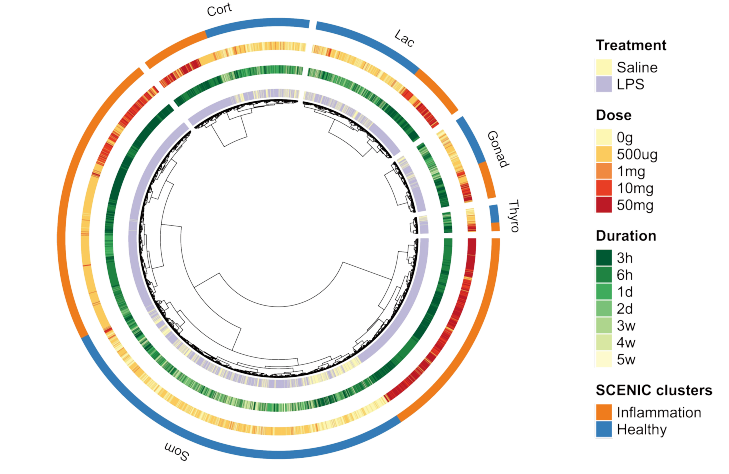
\includegraphics[width=\linewidth]{figs/expr-res3.png}
    \end{column}
  \end{columns}
\end{frame}

\begin{frame}{分析不同细胞在炎症状态下的基因表达差异}
  \begin{columns}
    \begin{column}{.5\linewidth}
      \begin{itemize}
        \item 我们进一步分析了垂体中不同细胞在两种状态下的差异表达基因集合。
        \item 同处于炎症状态,垂体中不同细胞应对炎症所做出的基因表达调整并不一致。
        \item 在中枢神经内分泌系统处于炎症状态时,垂体内各类细胞会采取不同的应激方式,组成一个调节炎症反应的复杂系统。
      \end{itemize}
    \end{column}

    \begin{column}{.5\linewidth}
      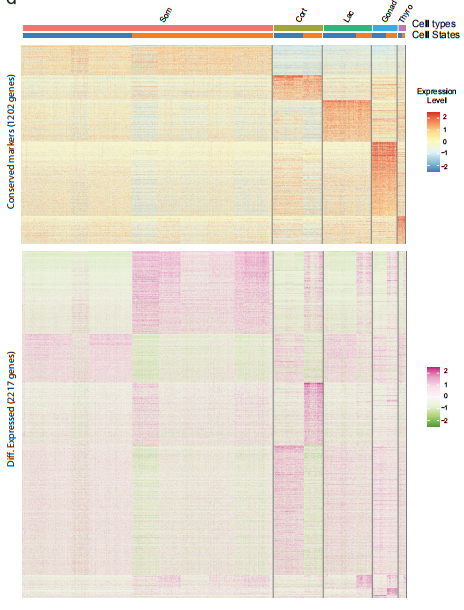
\includegraphics[width=\linewidth]{figs/expr-res4.png}
    \end{column}
  \end{columns}
\end{frame}

\begin{frame}{分析导致炎症状态的转录因子}
  \begin{columns}
    \begin{column}{.5\linewidth}
      \begin{itemize}
        \item 寻找具备双峰分布或者重尾分布的转录因子,对其自适应二值化后可以很好地与SCENIC标签匹配起来。
        \item Stat、Irf以及Nfkb等转录因子家族没有展现出细胞种类的特异性,是垂体参与中枢神经内分泌炎症调节过程中的Master Regulator Genes(MRs)。
      \end{itemize}
    \end{column}

    \begin{column}{.5\linewidth}
      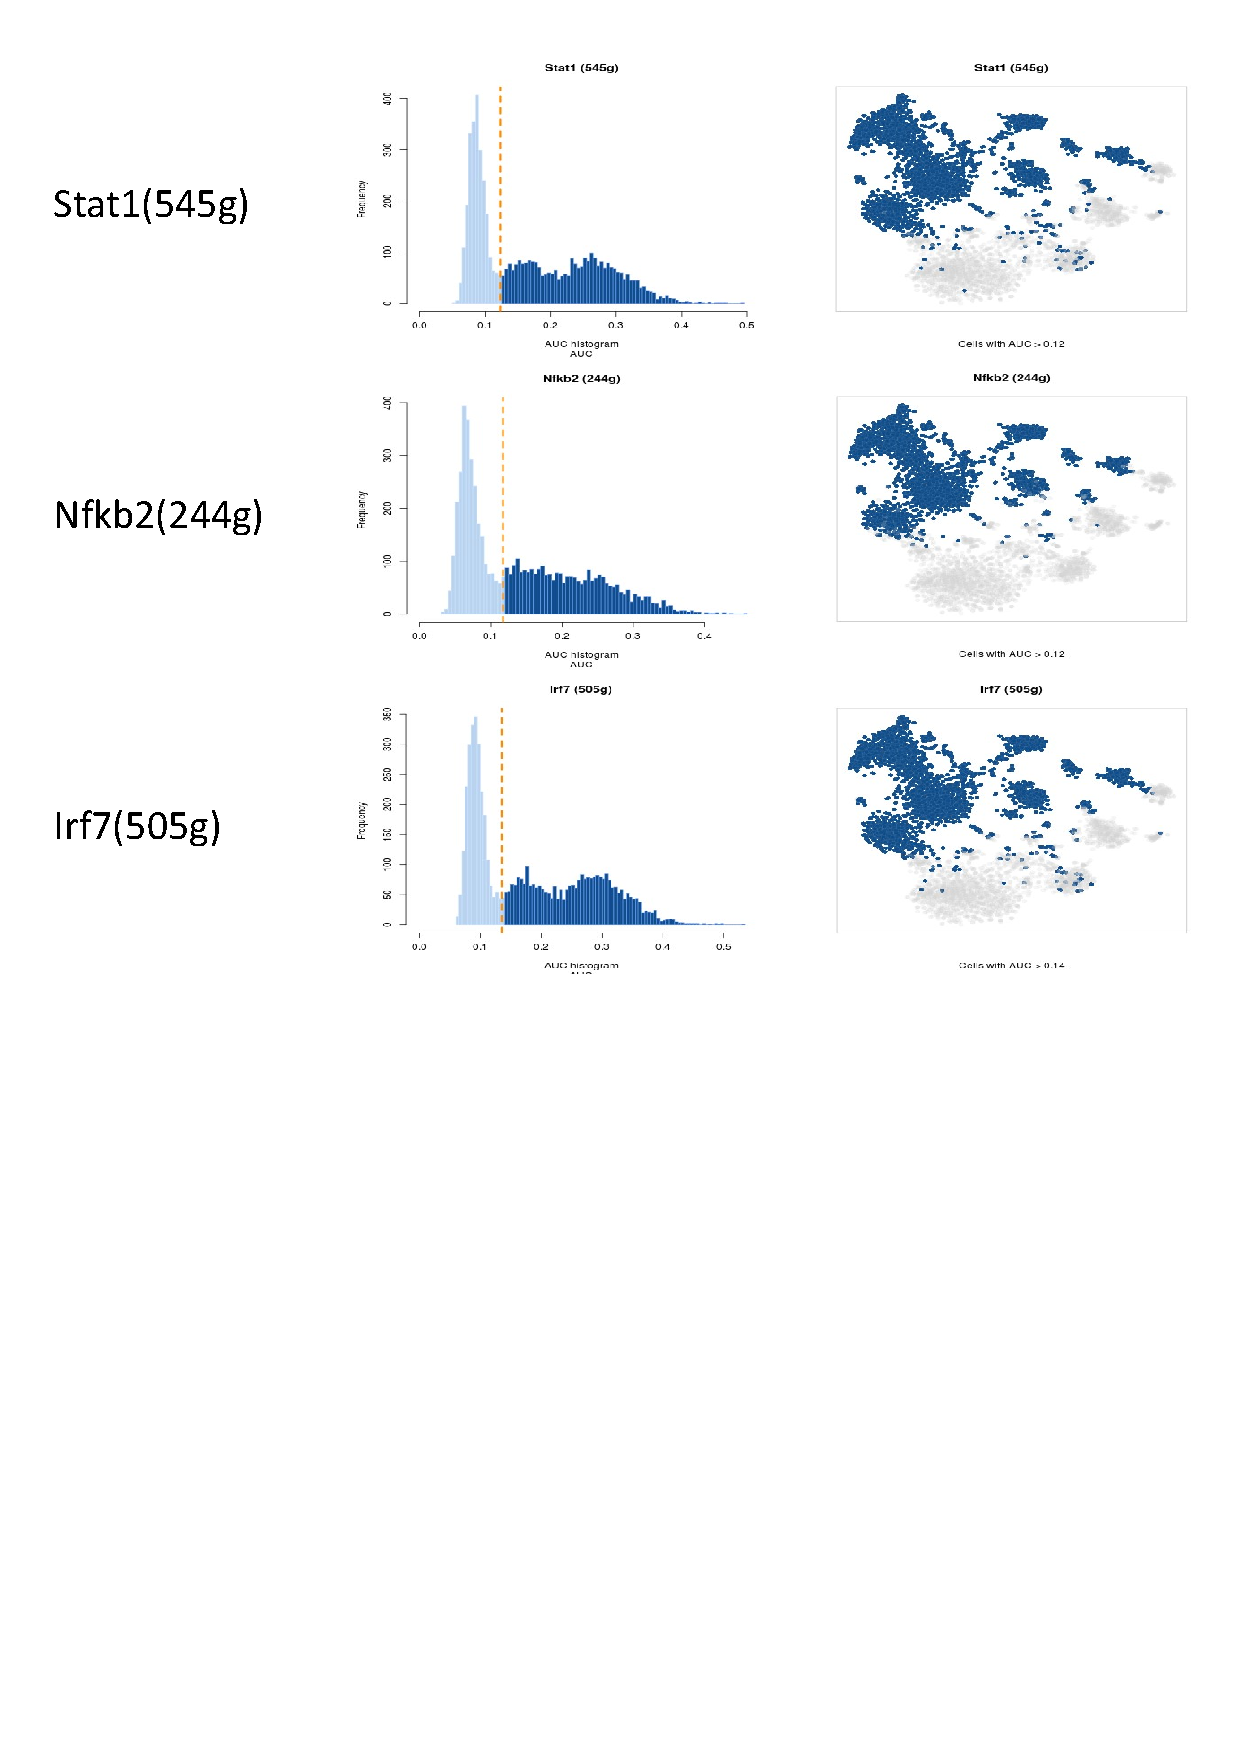
\includegraphics[width=\linewidth]{figs/expr-res5.pdf}
    \end{column}
  \end{columns}
\end{frame}

\section{总结与展望}

\begin{frame}{主要贡献}
  \begin{itemize}
    \item 建立了一个涉及多种免疫刺激剂、多尺度给药剂量与恢复时程的小鼠炎症模型,并在单细胞水平上提供了其垂体细胞测序数据。
    \item 揭示了不同种类垂体细胞在参与中枢神经内分泌炎症调节的过程中的转录水平差异,表明其在炎症调节过程中扮演不同的角色。
    \item 发现了一类在不同种类垂体细胞中统一表达的转录因子,表明其在垂体参与中枢神经内分泌炎症调节过程中的重要地位。
  \end{itemize}
\end{frame}

\begin{frame}{未来工作}
  \begin{itemize}
    \item 在给以小鼠$TNF-\alpha$刺激之后,其部分垂体细胞在经历UMAP可视化降维之后,呈现出与其他炎症状态细胞相分离的现象。
    \item 进一步探讨面对不可恢复炎症刺激与可恢复炎症刺激时垂体细胞在转录水平上的差异,揭示由健康(healthy)状态向这两种炎症(inflammation)状态转变的关键转录因子。
  \end{itemize}
\end{frame}

\section{致谢}

\begin{frame}{Thanks}
  \begin{center}
    {\Huge Thanks!}
  \end{center}
  \begin{itemize}
    \item 指导老师:蔡朝晖、罗敏敏
    \item 答辩学生:郑晖(2017300030039)
  \end{itemize}
\end{frame}

\end{document}
